\documentclass{scrartcl}	% classe article di KOMA
\reversemarginpar
\newcommand{\MarginDate}[1]{\marginpar{\raggedleft\itshape\small#1}}
%\usepackage[latin1]{inputenc}	% la codifica di input
%\usepackage[T1]{fontenc}	% la codifica dei font
\usepackage[LabelsAligned]{currvita}	% un buon pacchetto per CV
\usepackage[nochapters]{classicthesis} % stile ClassicThesis
\usepackage{url}	% per gli indirizzi Internet
\renewcommand{\cvheadingfont}{\LARGE\color{Maroon}}
\renewcommand{\cvlistheadingfont}{\large}
\renewcommand{\cvlabelfont}{\qquad}
%Setup hyperref package, and colours for links, text and headings
\usepackage{hyperref}		
\hypersetup{colorlinks,breaklinks,
	    urlcolor=Maroon, 
	    linkcolor=Maroon}
\usepackage{eurosym}
\usepackage{graphicx}
\usepackage{float}
\usepackage{ragged2e}
\newlength{\datebox}\settowidth{\datebox}{Summer 2007}

\newcommand{\NewWorkExperience}[3]{\noindent\hangindent=2em\hangafter=0 \parbox{\datebox}{\textit{#1}}\hspace{1.5em} #2 #3%
\vspace{0.5em}}

\newcommand{\Description}[1]{\hangindent=2em\hangafter=0\noindent\raggedright\footnotesize{#1}\par\normalsize}
\newcommand{\Sep}{\vspace{2em}}
\begin{document}
\thispagestyle{empty}
\begin{cv}{\spacedallcaps{Vojtech Vitek}}


%%% Contact %%%
\vspace{1.5em}
\noindent\spacedlowsmallcaps{Contact}
\vspace{0.5em}

\NewWorkExperience{E-mail}{\href{mailto:vojtech.vitek@gmail.com}{vojtech.vitek@gmail.com}}{}

\NewWorkExperience{Phone}{+1-647-773-0468}{}

\NewWorkExperience{Location}{Toronto, ON, Canada}{}

\NewWorkExperience{LinkedIn}{\href{http://www.linkedin.com/in/vojtechvitek}{linkedin.com/in/vojtechvitek}}{}

\NewWorkExperience{GitHub}{\href{https://github.com/VojtechVitek}{github.com/VojtechVitek}}{}

\NewWorkExperience{StackOverflow}{\href{http://stackoverflow.com/users/385548/vojtech-vitek}{stackoverflow.com/users/385548}}{}

\MarginDate{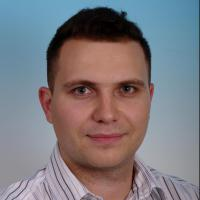
\includegraphics[width=10em]{CV.jpg}}


%%% Summary %%%
\vspace{1.0em}
\noindent\spacedlowsmallcaps{Summary}
\vspace{0.5em}

\Description{\MarginDate{}I'm friendly and positively thinking backend developer with strong Linux background. I enjoy working with Golang, Docker, Kubernetes, Bash, AngularJS and React.js. Besides my passion for IT, I like traveling and meeting new people. I do several sports actively and I'm musician. I've relocated from Prague (Czech Rep.) to Toronto in 2014 to challenge myself and start a new life experience. I'm interested in relocating to the U.S. in the near future. I'm open to new challenges and opportunities.
}

%%% Work experience %%%
\vspace{1.5em}
\noindent\spacedlowsmallcaps{Work Experience}
\vspace{0.5em}

\NewWorkExperience{2 months}{Software Engineer at Pressly}

\Description{\MarginDate{Golang Backend Development}\textit{Feb 2015 - Present}\newline Responsible for designing and maintaining high available Golang REST API microservices with MongoDB, PostgreSQL and LedisDB storages. Responsible for Docker deployments on EC2. \href{http://www.pressly.com}{www.pressly.com}
\begin{itemize}
  \item Golang, REST, MongoDB, PostgreSQL, LedisDB, Travis CI
  \item Docker, Ubuntu, EC2
\end{itemize}
}

\Sep

\NewWorkExperience{2.5 years}{Software Engineer at Red Hat}

\Description{\MarginDate{Golang Backend Development \& PHP Expert}\textit{Aug 2012 - Feb 2015}\newline Developing OpenShift 3 (Golang), the next generation PaaS built on top of Google Kubernetes and Docker containers. Responsible for Developer Experience and PHP and Zend Server environments. \href{http://www.openshift.com}{www.openshift.com}
\begin{itemize}
  \item Golang, REST, Bash, PHP, Zend Server, MongoDB, Etcd, Jenkins
  \item Docker, Kubernetes, EC2, RHEL, Atomic, CentOS, Fedora
\end{itemize}
}

\Sep

\NewWorkExperience{2.5 years}{Associate Software Engineer at Red Hat}

\Description{\MarginDate{GNU/Linux Software Maintenance}\textit{Oct 2010 - Jul 2012}\newline Fedora/RHEL package maintainer. Responsible for dozen core GNU/Linux applications, most notably PHP 5.x + PECLs, Rsync, GNU Awk, tcsh, gzip, xinetd, less and sed. \href{http://www.redhat.com}{www.redhat.com}
\begin{itemize}
  \item RPM, Bash, C/C++, PHP 5.x, Awk
\end{itemize}
}

\Sep

\NewWorkExperience{4.5 years}{SysAdmin \& PHP Devel. at Blue Solutions}

\Description{\MarginDate{Linux Administration, Drupal Development}\textit{2009 - 2013}\newline Side job. Co-founder of dot-com company focusing on robust web portals and e-shops. Responsible for VM-based CentOS server infrastructure. Developing custom Drupal 6/7 modules. \href{http://www.modryweb.cz/}{www.modryweb.cz}
\begin{itemize}
  \item CentOS 6, DNS, Varnish, Nginx, PHP-FPM, OPcache, Redis, MySQL
  \item Drupal 7, Drupal Commerce, JavaScript, jQuery
\end{itemize}
}

\Sep


%%% EDUCATION %%%
\vspace{1.5em}
\noindent\spacedlowsmallcaps{Education}
%\vspace{0.5em}

\NewWorkExperience{2007 - 2011}{Brno University of Technology,}{Czech Rep.}

\Description{\MarginDate{Bachelor's Degree}Information Technology - Bachelor's Degree. Graduated with ``Native Code Browser Extensions'' Bachelor thesis, focused on front-end browser extensions, C/C++ NPAPI plugins for Mozilla Firefox, Google Chrome and Opera browsers and applications sandboxed using Native Client. \newline\newline
\MarginDate{Outstanding Results}Placed in top 5\% students and received several scholarships for outstanding academic results. \href{http://www.fit.vutbr.cz/}{www.fit.vutbr.cz}
\newline\newline
\MarginDate{Exchange~Studies}Erasmus exchange studies at Yildiz Technical University, Istanbul, Turkey, focused on Unix operating systems and Oracle database storage technologies. Gained ``A'' grades in all courses taken and received scholarship for outstanding academic results. \href{http://www.yildiz.edu.tr/en/}{www.yildiz.edu.tr/en/}
\newline\newline
\MarginDate{Network Academy Research}Responsible for developing software tools and drivers for custom High-speed 100G Network Cards, CentOS/Debian server infrastructure and RPM/DEB packaging. \href{http://www.liberouter.org}{www.liberouter.org}
}


%%% Certifications %%%
\vspace{1.5em}
\noindent\spacedlowsmallcaps{Certifications}
%\vspace{0.5em}

\Description{\begin{itemize}
 \item Red Hat Certified System Administrator (RHCSA), 120-019-294
 \item Red Hat Project Management Academy, 2012
\end{itemize}
}


%%% Awards %%%
\vspace{1.5em}
\noindent\spacedlowsmallcaps{Awards \& International Scholarships}
%\vspace{0.5em}

\Description{\begin{itemize}
 \item 2011, Winner of the CZ.NIC VIP 3 Open-Source Competition
 \item 2010, Winner of the CZ.NIC VIP 2 Open-Source Competition
 \item 2009, Winner of the Student EEICT Academy Project Competition
 \item 2009, Winner of the GE Foundation International Scholarship for the 15 most accomplished students of technical universities in the Central and Eastern Europe
\end{itemize}
}

\enlargethispage{\baselineskip}
\end{cv}
\end{document}
